% The text of the two acmart fixtures, with a raster figure, a drawn figure, a table over the text width, a listing,
% footnotes, and long URLs, each placed as the template intends.
\begin{abstract}
Flaky tests pass and fail on the same code. This paper ranks the failures of a build by the
chance that each failure is flaky. On 4,210 failures of ten projects, the ranking places the
flaky failure first in 71\% of the builds.
\end{abstract}

\begin{CCSXML}
<ccs2012>
<concept>
<concept_id>10011007.10011074.10011099.10011102.10011103</concept_id>
<concept_desc>Software and its engineering~Software testing and debugging</concept_desc>
<concept_significance>500</concept_significance>
</concept>
</ccs2012>
\end{CCSXML}
\ccsdesc[500]{Software and its engineering~Software testing and debugging}
\keywords{flaky tests, regression testing, continuous integration}

\maketitle

\section{Introduction}
\lipsum[1]
The study builds on the public logs of the projects, such as
\url{https://github.com/apache/commons-lang/actions/workflows/maven.yml?query=branch%3Amaster+event%3Apush}
and the issue tracker at
\url{https://issues.apache.org/jira/projects/LANG/issues/LANG-1700?filter=allopenissues}.\footnote{The
build logs come from \url{https://api.github.com/repos/apache/commons-lang/actions/runs?per_page=100&page=1}.}
\lipsum[2]

\begin{figure}[t]
\centering
\includegraphics[width=\linewidth]{example-image-16x9.png}
\caption{A build page as a raster image of the full text width.}
\Description{A gray placeholder image.}
\label{fig:raster}
\end{figure}

\section{Approach}
\lipsum[3]
Figure~\ref{fig:raster} shows a build page, Figure~\ref{fig:pipeline} the stages of the
ranking, and Listing~\ref{lst:test} a flaky test.\footnote{A second footnote with a long address,
\url{https://docs.github.com/en/actions/using-workflows/events-that-trigger-workflows\#workflow_run}.}

\begin{figure}[t]
\centering
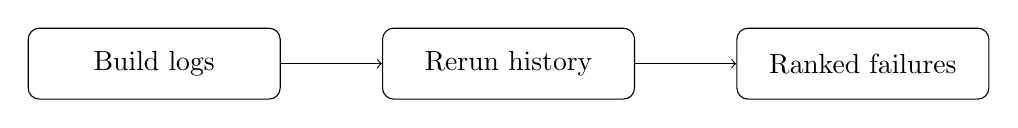
\begin{tikzpicture}[stage/.style={draw, rounded corners, minimum width=3.2cm, minimum height=0.9cm}]
\node[stage] (a) at (0,0) {Build logs};
\node[stage] (b) at (4.5,0) {Rerun history};
\node[stage] (c) at (9,0) {Ranked failures};
\draw[->] (a) -- (b);
\draw[->] (b) -- (c);
\end{tikzpicture}
\caption{The stages of the ranking.}
\Description{Three boxes joined by arrows.}
\label{fig:pipeline}
\end{figure}

\begin{lstlisting}[caption={A test that depends on the order of the suite.}, label={lst:test}]
@Test
public void readsSharedCache() {
    assertEquals(0, SharedCache.getInstance().size());
    SharedCache.getInstance().put("key", computeExpensiveValueFromTheNetwork("https://example.org/a/long/path"));
}
\end{lstlisting}

\section{Evaluation}
\lipsum[4]
Table~\ref{tab:ranks} gives the ranks per project.

\begin{table}[t]
\caption{Rank of the flaky failure per project and method}
\label{tab:ranks}
\begin{tabular*}{\linewidth}{@{\extracolsep{\fill}}lrrrrrrrrrr@{}}
\toprule
Method & lang & guava & jsoup & spring & netty & kafka & flink & hadoop & hbase & Total \\
\midrule
Ranking & 61 & 133 & 30 & 140 & 88 & 120 & 95 & 160 & 110 & 937 \\
Rerun order & 33 & 70 & 16 & 77 & 41 & 64 & 52 & 85 & 62 & 500 \\
\bottomrule
\end{tabular*}
\end{table}

\lipsum[5-7]

\section*{Data Availability}
The data and scripts are available at
\url{https://anonymous.4open.science/r/flaky-ranking-replication-package-2027/README.md}.

\begin{thebibliography}{2}
\bibitem[Lam et~al.(2019)]{lam} Wing Lam, Reed Oei, August Shi, Darko Marinov, and Tao Xie. 2019.
iDFlakies: A Framework for Detecting and Partially Classifying Flaky Tests. In \emph{Proc. ICST}. 312--322.
\bibitem[GitHub(2026)]{gh} GitHub. 2026. Events that trigger workflows.
\url{https://docs.github.com/en/actions/writing-workflows/choosing-when-your-workflow-runs/events-that-trigger-workflows}
\end{thebibliography}
